\section{Convergence Theory}
\label{ch:convergence}
 
Part~3 has so far been constructive. Chapter~4 built a smooth surrogate
for the chance constraint, Chapter~5 redesigned it to err only on the
safe side, and both chapters validated their constructions empirically
on problems whose answers are known. What neither chapter could supply
is the statement that elevates a construction to a method: the guarantee
that solving the approximated problem is, in the limit of data, the same
as solving the true one. That statement exists. The convergence theory
of \citet{schuster2025} proves three theorems which together establish
that the KDE-approximated chance-constrained problem is a well-posed
approximation of the original: the approximation is exact where the
constraint is inactive, the limits of approximate solutions are true
solutions, and under a sharp-minimum condition such limits exist. This
chapter is the theoretical center of the thesis. It states the gap the
theory fills and why density-estimator consistency alone cannot fill it
(\cref{sec:gap}), fixes the setting and assumptions
(\cref{sec:setupassump}), develops each theorem with its statement,
proof architecture, and practical meaning
(\cref{sec:thm1,sec:thm2,sec:thm3}), draws the boundary of what the
theory does and does not cover (\cref{sec:coverage}), and closes on the
structural gap between the two anchor papers of this thesis, which is
arguably the most important open problem in the field
(\cref{sec:anchorgap}).
 
\subsection{The Gap the Theory Fills}
\label{sec:gap}
 
The biased construction of Chapter~5 provides a safety guarantee by
construction: any feasible solution of the biased reformulation
satisfies the original chance constraint in expectation. It is essential
to recognize precisely what this guarantees and what it does not. It is
a statement about the \emph{feasibility of individual solutions}, made
at finite $N$; it says nothing about whether the optimizer, in
certifying and comparing such solutions, is converging to the right one.
A method could be safe at every $N$ and still be solving, indefinitely,
a problem whose minimizer differs substantially from the minimizer of
the true problem. Safety and correctness are different properties, and Part~3 has
so far delivered only the first.
 
The deeper question is therefore the one this chapter answers: as the
sample size $N$ grows, do solutions of the KDE-approximated problem
converge to solutions of the true chance-constrained problem?
\citet{schuster2025} provides the first rigorous answer, and the key
insight that organizes the entire theory deserves to be stated before
any theorem is: \emph{density-estimator convergence does not
automatically imply optimizer convergence}. That the kernel estimate
converges to the true density has been known since \citet{parzen1962},
and Chapter~2 reviewed the classical theory in full; but an optimization
problem is not a density. Its solution is determined by the interaction
of an objective with the \emph{boundary} of a feasible set, and a
sequence of converging constraint functions can, in principle, produce
feasible sets whose minimizers behave badly: solutions can fail to
exist, can wander without converging, or can converge to limits that are
infeasible or suboptimal for the true problem. A separate argument is
needed to transfer convergence of the constraint approximation to
convergence of the solution, and constructing that argument, in three
theorems of increasing reach, is exactly what \citet{schuster2025} does.
\Cref{fig:chain} displays the architecture the rest of this chapter
walks through: a statistical foundation inherited from classical KDE
theory, two analytical engines, and the three theorems they power.
 
\begin{figure}[t]
  \centering
  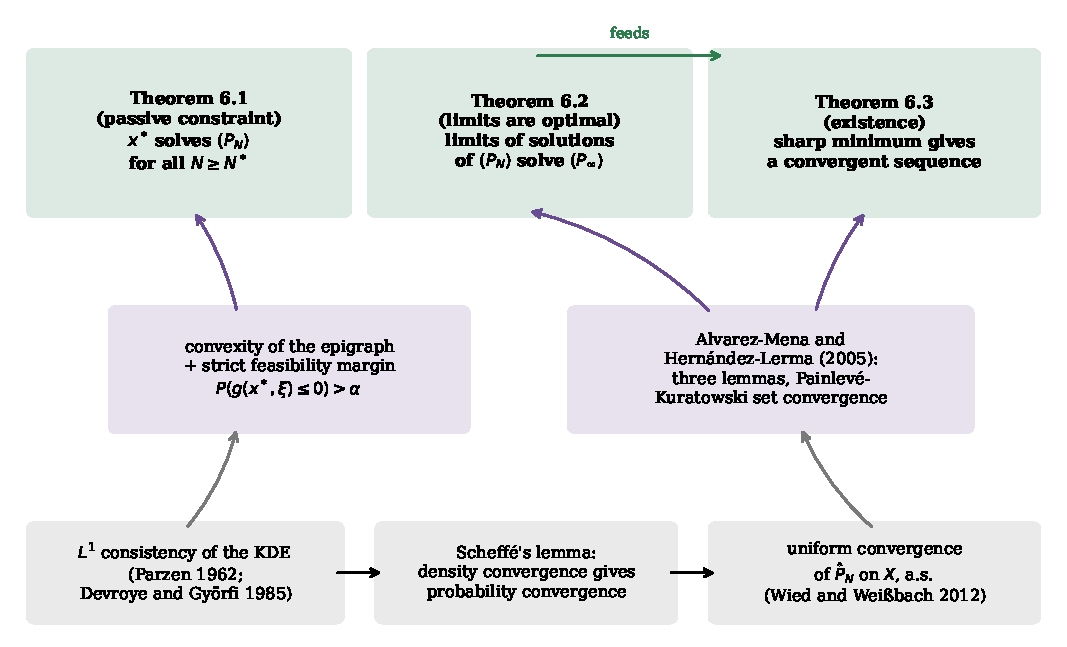
\includegraphics[width=\textwidth]{kap05/figures/fig_chain.pdf}
  \caption{The architecture of the convergence theory of
  \citet{schuster2025}. The statistical foundation (bottom row) is
  classical: $L^1$ consistency of the kernel estimator, upgraded to
  probability convergence by Scheff\'e's lemma and to almost-sure
  uniform convergence on the feasible set under the conditions surveyed
  by \citet{wied2012}. Two analytical engines (middle row) convert
  statistical convergence into optimization statements: a
  convexity-of-epigraph argument with a strict feasibility margin, and
  the optimization-convergence theorem of \citet{alvarezmena2005}
  verified through three lemmas. The three theorems (top row) divide the
  labor: exactness where the constraint is passive, optimality of limits,
  and existence of convergent solution sequences.}
  \label{fig:chain}
\end{figure}
 
\subsection{Setup and Assumptions}
\label{sec:setupassump}
 
The theory is formulated at a level of generality worth pausing on,
because it is part of the result. The decision space is not assumed
finite-dimensional: \citet{schuster2025} works in a Banach space, which
is precisely the generality required for the optimal control ambitions
of this thesis, where decisions are trajectories before they are
discretized. The standing assumptions are collected once.
 
\begin{assumption}[Setting of \citealp{schuster2025}]
\label{ass:setting}
$V$ is a Banach space and $X \subseteq V$ is closed and nonempty. The
objective $f$ is convex and monotonically increasing. The random
parameter $\xi$ has an absolutely continuous distribution, so that for
every $x \in X$ the pushforward density $\rho_{g(x)}$ of the residual
vector $g(x,\xi) \in \R^m$ exists.
\end{assumption}

Under \cref{ass:setting} the chance constraint is the statement that the
pushforward density places mass at least $\alpha = 1-\varepsilon$ on the
safe orthant,
\begin{equation}
  \Prob\bigl(g(x,\xi) \leq 0\bigr)
  \;=\; \int_{(-\infty,0]^m} \rho_{g(x)}(z)\, dz \;\geq\; \alpha ,
  \label{eq:pushforward}
\end{equation}
which the reader will recognize as the residual-space identity of
Chapter~4, here in its general $m$-dimensional form: the theory covers
joint constraints through the multivariate residual, and the scalar case
$m = 1$ of Chapters~4 and~5 is the special case used throughout this
thesis. The approximation replaces $\rho_{g(x)}$ by its kernel estimate
built from the residual samples $Y_i(x) = g(x,\xi_i)$, exactly the
estimator of Chapter~4, and the pair of problems whose relationship the
theory governs is
\begin{align}
  (P_\infty):\quad
  &\minimize_{x \in X} f(x)
  \quad\text{subject to}\quad
  \Prob\bigl(g(x,\xi) \leq 0\bigr) \geq \alpha ,
  \label{eq:pinf}\\
  (P_N):\quad
  &\minimize_{x \in X} f(x)
  \quad\text{subject to}\quad
  \hat{P}_N\bigl(g(x,\xi) \leq 0\bigr) \geq \alpha .
  \label{eq:pn}
\end{align}
Every theorem below is a statement about how the solutions of $(P_N)$
relate to those of $(P_\infty)$, almost surely with respect to the
sampling of $\xi_1, \xi_2, \dots$, and the three theorems are numbered
here as \cref{thm:passive,thm:limits,thm:existence}, corresponding to
Theorems~3.1, 3.2, and~3.3 of \citet{schuster2025} respectively.
 
\subsection{The Passive Constraint Case}
\label{sec:thm1}
 
The first theorem settles the regime in which the chance constraint, at
the optimum, is not doing any work.
 
\begin{theorem}[Passive constraint; Theorem 3.1 of \citealp{schuster2025}]
\label{thm:passive}
Let $x^*$ solve $(P_\infty)$ with the chance constraint strictly
inactive, $\Prob(g(x^*,\xi) \leq 0) > \alpha$. Then there exists $N^*$
such that $x^*$ also solves $(P_N)$ for all $N \geq N^*$, almost surely.
\end{theorem}
 
\emph{Proof architecture.} The argument runs along the bottom-left of
\cref{fig:chain}. The $L^1$ consistency of the kernel estimator
\citep{parzen1962,devroye1985} controls the integrated error of the
density estimate; Scheff\'e's lemma \citep{scheffe1947} converts $L^1$
convergence of densities into convergence of the probabilities they
induce, so that $|\hat{P}_N - \Prob|$ at $x^*$ falls, almost surely,
below the strict feasibility margin
$\gamma = \Prob(g(x^*,\xi) \leq 0) - \alpha > 0$ for all $N$ beyond some
$N^*$. From that point on, $x^*$ remains feasible for every $(P_N)$, and
a convexity-of-epigraph argument transfers the solution property: a
point that is optimal among a larger feasible set and feasible for the
smaller one is optimal for the smaller one as well.
 
\emph{Practical meaning.} Where the chance constraint does not bind at
the optimum, the KDE approximation introduces no error at all for large
samples; the constraint is effectively transparent, and the problem
behaves locally like the deterministic problem it would be without the
constraint. \Cref{fig:passive} draws the mechanism: the margin $\gamma$
is a fixed buffer, the uniform estimation error is a tube around the
true probability that shrinks with $N$, and once the tube fits inside
the buffer the approximation can no longer disturb the solution. The
theorem is the formal license for an instinct every practitioner has:
approximation error only matters where the constraint matters.

\begin{figure}[t]
  \centering
  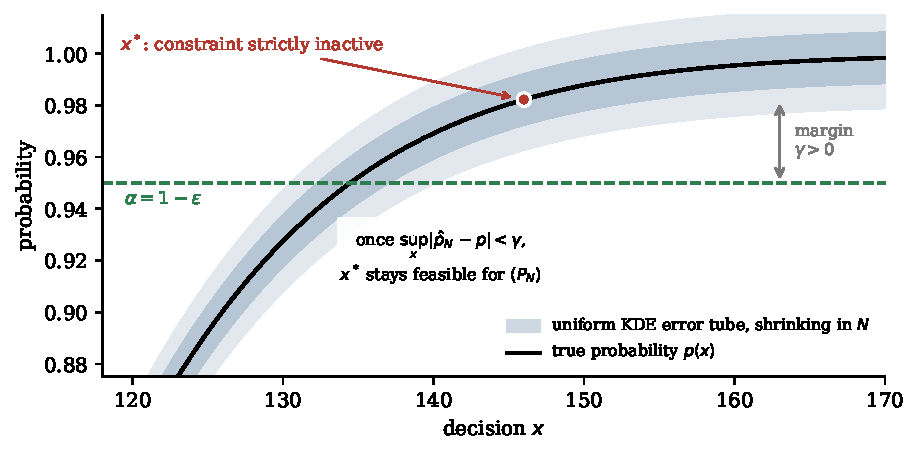
\includegraphics[width=0.86\textwidth]{kap05/figures/fig_passive.pdf}
  \caption{The mechanism of \cref{thm:passive}, drawn on the dispatch
  problem's probability curve. At a solution $x^*$ where the chance
  constraint is strictly inactive, the feasibility margin
  $\gamma = \Prob(g(x^*,\xi) \leq 0) - \alpha$ is a fixed positive
  buffer. The KDE error is a tube around the true probability that
  shrinks almost surely as $N$ grows; once
  $\sup_x |\hat{p}_N - p| < \gamma$, the point $x^*$ is feasible for
  every approximated problem and, by the epigraph argument, solves it.}
  \label{fig:passive}
\end{figure}
 
\subsection{Limits of Approximate Solutions Are Optimal}
\label{sec:thm2}
 
The second theorem addresses the regime the first one excludes, the one
that matters most in practice: the constraint binds, the approximated
solutions move with $N$, and the question is where they are allowed to
go.

\begin{theorem}[Limits are optimal; Theorem 3.2 of \citealp{schuster2025}]
\label{thm:limits}
Suppose the kernel estimate converges almost surely uniformly for every
$x \in X$. If $(x_N)$ is a convergent sequence of solutions of $(P_N)$,
then its limit solves $(P_\infty)$, almost surely.
\end{theorem}
 
\emph{Proof architecture.} This is the deepest of the three results, and
its proof is an exercise in verifying the hypotheses of a general
optimization-convergence theorem due to \citet{alvarezmena2005}, which
gives conditions under which minimizers of a sequence of problems
converge to minimizers of a limit problem. \citet{schuster2025}
establishes the three required conditions through three lemmas. The
first upgrades the statistical foundation: uniform convergence of the
kernel estimate yields uniform convergence of the constraint function
$\hat{P}_N$ to $\Prob$ on $X$. The second translates constraint
convergence into geometry: the admissible sets of $(P_N)$ converge to
the admissible set of $(P_\infty)$ in the Painlev\'e-Kuratowski sense,
the notion of set convergence under which limits of feasible points are
feasible. The third closes the loop from the other side: every feasible
point of the limit problem can be approached by a sequence of points
feasible for the approximating problems, so the approximations do not
silently exclude parts of the true feasible set. With the three
conditions in place, the theorem of \citet{alvarezmena2005} delivers the
conclusion.
 
\emph{Practical meaning.} Whatever the approximated problems converge
to, it is a true solution: the optimizer is approaching the right
answer, not an artifact of the smoothing. The theorem converts the
empirical convergence plots that this thesis produces in Part~4 from
suggestive pictures into evidence about $(P_\infty)$ itself, because it
guarantees that the plateau such plots approach is the true optimum and
not an artifact of the approximation. What the theorem deliberately
does not assert is that a convergent sequence exists; it is a statement
about limits, conditional on their existence. Closing that gap is the
third theorem's job, and the division of labor between
\cref{thm:limits,thm:existence} is itself instructive: optimality of
limits and existence of limits are separate mathematical events,
requiring separate hypotheses.

\subsection{Existence of a Convergent Solution Sequence}
\label{sec:thm3}
\begin{theorem}[Existence; Theorem 3.3 of \citealp{schuster2025}]
\label{thm:existence}
Suppose $x^*$ is the unique solution of $(P_\infty)$ and satisfies a
sharp-minimum condition: there exist $\bar{\varepsilon}, \delta > 0$
such that $f(x) > f(x^*) + \bar{\varepsilon}$ for every feasible $x$
outside the ball $B_\delta(x^*)$. Then a convergent sequence of
solutions of the approximated problems exists, almost surely.
\end{theorem}
 
\emph{Proof architecture.} The sharp-minimum condition is exactly what
forbids the failure mode that \cref{thm:limits} could not exclude. If
near-optimal objective values were available far from $x^*$, the
approximated solutions could achieve them and wander indefinitely;
the growth condition makes every such excursion expensive, and combined
with the set-convergence machinery of \cref{sec:thm2} it forces the
solution sequence to be Cauchy, hence convergent.
\Cref{fig:sharpmin} contrasts the two geometries: under a sharp minimum
the approximate solutions are trapped in a shrinking neighborhood of
$x^*$; in a shallow valley, nothing prevents them from drifting between
distant near-optimal points.
 
\emph{Practical meaning.} The conditions under which the full theory
operates are not exotic, and \citet{schuster2025} makes both halves of
that claim concrete. On the geometry side, strict convexity of the
objective already implies both the uniqueness of $x^*$ and the growth
condition, so the hypothesis of \cref{thm:existence} is met by a large
and recognizable problem class. On the statistical side, the uniform
convergence that \cref{thm:limits,thm:existence} require is not an
abstract wish: a Gaussian product kernel with a diagonal bandwidth
matrix, under the classical bandwidth conditions and uniform continuity
of the true density, is identified as a concrete realization that
guarantees it, drawing on the consistency conditions surveyed by
\citet{wied2012} and the $L^1$ theory of \citet{devroye1985}. The
theory's assumptions can be discharged by objects this thesis already
uses.

\begin{figure}[t]
  \centering
  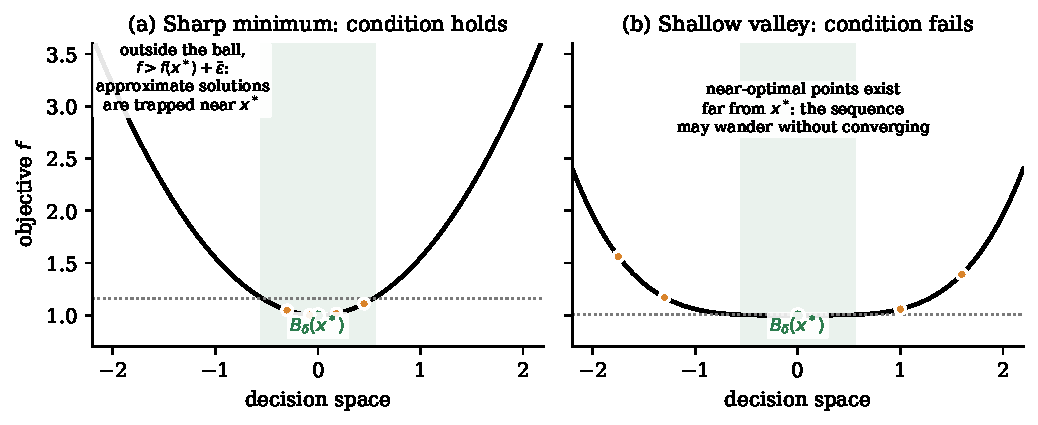
\includegraphics[width=\textwidth]{kap05/figures/fig_sharpmin.pdf}
  \caption{Why \cref{thm:existence} needs the sharp-minimum condition.
  (a) When the objective grows by at least $\bar{\varepsilon}$ outside
  the ball $B_\delta(x^*)$ (shaded), every approximate solution
  (orange) with near-optimal value is forced into the ball, and the
  set-convergence machinery makes the sequence Cauchy. (b) In a shallow
  valley the condition fails: near-optimal points exist far from $x^*$,
  and approximate solutions may alternate between them without
  converging, even though, by \cref{thm:limits}, any limit they did have
  would be optimal. Strict convexity of $f$ implies the geometry of
  panel (a).}
  \label{fig:sharpmin}
\end{figure}
 
\subsection{What the Theory Does and Does Not Cover}
\label{sec:coverage}
 
Taken together, the three theorems deliver the two assets this thesis
claims from them. The first is mathematical credibility: the KDE
approach is not a heuristic that happens to work but an asymptotically
consistent method, with the consistency proven at the level that
matters, the optimization problem, not merely the estimator inside it.
The second is precision about conditions: the theory identifies exactly
what convergence costs, namely uniform convergence of the estimate on
the feasible set, plus either a passive constraint or a sharp minimum,
and it exhibits concrete, standard objects that pay the cost. A reader
of Chapters~4 and~5 now knows not only how to build the reformulation
but when to trust it.
 
Intellectual honesty about the boundary is equally part of the asset,
and four items lie beyond it. There are, first, \emph{no convergence
rates}: the theory guarantees that the optimization error vanishes but
not how fast, and no theorem links the kernel's bias-variance behavior
to the decay of $|f(x_N) - f(x^*)|$ or $\|x_N - x^*\|$;
\citet{schuster2025} explicitly flags this as open.
\Cref{fig:empconv} makes the gap tangible: on the dispatch problem the
optimization error decays along a clean empirical power law of slope
roughly $-0.46$, a regular behavior that no available theorem
currently predicts. Second, the theorems cover the \emph{unbiased} estimator of
Chapter~4; whether and how they extend to the biased construction of
Chapter~5 is open, a point developed in \cref{sec:anchorgap}. Third, the
results lean on convexity of the objective, while the trajectory
optimization problems of Part~4 are non-convex; comparable guarantees
for the non-convex case do not exist. Fourth, the theory is asymptotic
through and through: unlike the scenario approach of Chapters~2 and~3,
it offers no $N$-dependent probability that a computed solution is
feasible for the true problem. These four boundaries are not defects of
the theory; they are its honest perimeter, and they define precisely
where the experimental program of Part~4 carries the burden of evidence
that mathematics does not yet carry.

\begin{figure}[t]
  \centering
  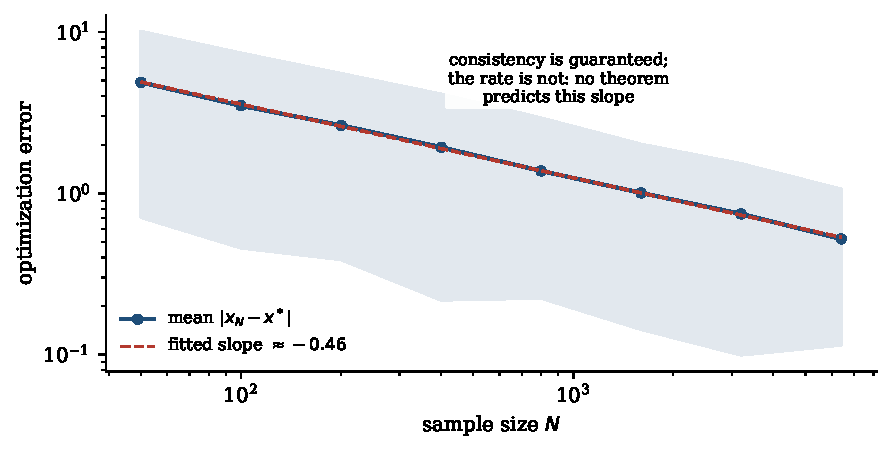
\includegraphics[width=0.84\textwidth]{kap05/figures/fig_empconv.pdf}
  \caption{Consistency without rates. Mean optimization error
  $|x_N - x^*|$ of the unbiased KDE solution on the dispatch problem
  ($500$ trials per sample size, band is $10$th-to-$90$th percentiles),
  on logarithmic axes. The error follows a clean empirical power law of
  slope $\approx -0.46$, but the convergence theory guarantees only that
  the error vanishes; no theorem predicts the slope. Quantifying this
  rate, and its dependence on the bandwidth rule, is the most important
  open problem the anchor papers leave}
  \label{fig:empconv}
\end{figure}
 
\subsection{The Gap Between the Two Anchor Papers}
\label{sec:anchorgap}
 
One observation deserves to close Part~3's theoretical development,
stated as plainly as its importance warrants. The two anchor papers of
this thesis work with the same high-level idea from opposite directions,
and their results do not yet meet. \citet{keil2021} builds a
\emph{biased} integrated kernel that dominates the indicator, securing a
finite-sample safety guarantee, but proves no convergence of the
resulting optimizers. \citet{schuster2025} proves convergence of the
optimizers, but for the \emph{unbiased} kernel density estimate, with no
safety guarantee at finite $N$. Neither paper's theorems cover the
other's construction: the engineering line has safety without proven
convergence, and the theoretical line has convergence without built-in
safety.
 
The open problem this leaves is easy to state and, in the judgment of
this thesis, arguably the most important one in the field: a unified
convergence
theory for the biased-KDE reformulation, establishing that the
conservative construction of Chapter~5 inherits the asymptotic
correctness of this chapter, ideally with rates. Its resolution would
fuse the two guarantees that applications actually need, safety at every
finite $N$ and correctness in the limit, into a single certified method.
This thesis does not claim to close that problem. What it does claim,
and delivers in Part~4, is the systematic empirical groundwork on which
a closure must rest: controlled experiments in which the biased and
unbiased reformulations are run side by side, across sample sizes,
bandwidths, and risk levels, on problems whose true solutions are
known, so that the conjectured convergence of the biased construction is
measured even where it is not yet proven. The theory of this chapter
tells us what such measurements mean; the gap between the anchors tells
us why they are worth making.